\subsection{Abstract classes}
\label{subsec:library_of_transformations:type_level_transformations:abstract_classes}

\begin{figure}[H]
    \centering
    \begin{subfigure}{0.45\textwidth}
        \centering
        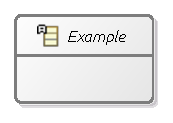
\includegraphics{images/05_library_of_transformations/02_type_level_transformations/02_abstract_classes/abstract_class_type.pdf}
        \caption{$Tm_{AbsClass}$ with $name = .\type{Example}$}
        \label{fig:library_of_transformations:type_level_transformations:abstract_classes:visualisation:ecore}
    \end{subfigure}
    \begin{subfigure}{0.45\textwidth}
        \centering
        % To use this figure in your LaTeX document
% import the package groove/resources/groove2tikz.sty
%
\begin{tikzpicture}[scale=\tikzscale,name prefix=test-]
\node[abstract_node] (n0) at (0.890, -0.830) {\ml{\textit{\textbf{Example}}}};

\end{tikzpicture}

        \caption{$TG_{AbsClass}$ with $name = .\type{Example}$}
        \label{fig:library_of_transformations:type_level_transformations:abstract_classes:visualisation:groove}
    \end{subfigure}
    \caption{Visualisation of the transformation of abstract classes}
    \label{fig:library_of_transformations:type_level_transformations:abstract_classes:visualisation}
\end{figure}

This section defines a transformation that is very close to the previous transformation. In this section, an abstract class without any additional properties is defined. The Ecore model for defining an abstract class is given in the following definition:

\begin{defin}[Type model $Tm_{AbsClass}$]
\label{defin:library_of_transformations:type_level_transformations:abstract_classes:tmod_abstract_class}
Let $Tm_{AbsClass}$ be the type model containing an abstract class with identifier $name$. $Tm_{AbsClass}$ is defined as:
\begin{align*}
Class =\ &\{name\} \\
Enum =\ &\{\} \\
UserDataType =\ &\{\} \\
Field =\ &\{\} \\
\mathrm{FieldSig} =\ &\{\} \\
EnumValue =\ &\{\} \\
Inh =\ &\{\} \\
Prop =\ &\{[ \type{abstract}, name ]\} \\
Constant =\ &\{\} \\
\mathrm{ConstType} =\ &\{\}
\end{align*}
\isabellelref{tmod_abstract_class}{Ecore-GROOVE-Mapping-Library.AbstractClassType}
\end{defin}

\begin{thm}[Correctness of $Tm_{AbsClass}$]
\label{defin:library_of_transformations:type_level_transformations:abstract_classes:tmod_abstract_class_correct}
$Tm_{AbsClass}$ (\cref{defin:library_of_transformations:type_level_transformations:abstract_classes:tmod_abstract_class}) is a consistent type model in the sense of \cref{defin:formalisations:ecore_formalisation:type_models:type_model_consistency}.
\isabellelref{tmod_abstract_class_correct}{Ecore-GROOVE-Mapping-Library.AbstractClassType}
\end{thm}

A visual representation of $Tm_{AbsClass}$ with identifier $.\type{Example}$ can be seen in \cref{fig:library_of_transformations:type_level_transformations:abstract_classes:visualisation:ecore}. The correctness proof of $Tm_{AbsClass}$ is trivial, and therefore not included here. The proof can be found as part of the Isabelle validated proofs.

In order to make composing transformation functions possible, $Tm_{AbsClass}$ should be compatible with the type model it is combined with.

\begin{thm}[Correctness of $\mathrm{combine}(Tm, Tm_{AbsClass})$]
\label{defin:library_of_transformations:type_level_transformations:abstract_classes:tmod_abstract_class_combine_correct}
Assume a type model $Tm$ that is consistent in the sense of \cref{defin:formalisations:ecore_formalisation:type_models:type_model_consistency}. Then $Tm$ is compatible with $Tm_{AbsClass}$ (in the sense of \cref{defin:transformation_framework:type_models_and_type_graphs:combining_type_models:compatibility}) if:
\begin{itemize}
    \item The identifier of the class in $Tm_{AbsClass}$ is not yet an identifier for a class, enumeration type or user-defined data type in $Tm$;
    \item The identifier of the class in $Tm_{AbsClass}$ is not in the namespace of any class, enumeration type or user-defined data type in $Tm$;
    \item None of the identifiers in any class, enumeration type or user-defined data type in $Tm$ is in the namespace of the class in $Tm_{AbsClass}$.
\end{itemize}
\isabellelref{tmod_abstract_class_combine_correct}{Ecore-GROOVE-Mapping-Library.AbstractClassType}
\end{thm}

\begin{proof}
Use \cref{defin:transformation_framework:type_models_and_type_graphs:combining_type_models:tmod_combine_merge_correct}. It is possible to show that all assumptions hold. Now we have shown that $\mathrm{combine}(Tm, Tm_{AbsClass})$ is consistent in the sense of \cref{defin:formalisations:ecore_formalisation:type_models:type_model_consistency}.
\end{proof}

The definitions and theorems for a regular class within Ecore are now complete. 

\subsubsection{Encoding as node type}

A possible encoding for abstract classes in Ecore is using a node type in GROOVE. This node type will get a transformed identifier as name. The encoding corresponding to $Tm_{AbsClass}$ can then be represented as $TG_{AbsClass}$, defined in the following definition:

\begin{defin}[Type graph $TG_{AbsClass}$]
\label{defin:library_of_transformations:type_level_transformations:abstract_classes:tg_abstract_class_as_node_type}
Let $TG_{AbsClass}$ be the type graph containing a single node type which encodes an abstract class $name$. $TG_{AbsClass}$ is defined as:
\begin{align*}
NT =\ &\{\mathrm{ns\_\!to\_\!list}(name)\} \\
ET =\ &\{\} \\
\!\!\sqsubseteq\ =\ &\{(\mathrm{ns\_\!to\_\!list}(name), \mathrm{ns\_\!to\_\!list}(name))\} \\
abs =\ &\{\mathrm{ns\_\!to\_\!list}(name)\} \\
\mathrm{mult} =\ &\{\} \\
contains =\ &\{\}
\end{align*}
\isabellelref{tg_abstract_class_as_node_type}{Ecore-GROOVE-Mapping-Library.AbstractClassType}
\end{defin}

\begin{thm}[Correctness of $TG_{Class}$]
\label{defin:library_of_transformations:type_level_transformations:abstract_classes:tg_abstract_class_as_node_type_correct}
$TG_{AbsClass}$ (\cref{defin:library_of_transformations:type_level_transformations:abstract_classes:tg_abstract_class_as_node_type}) is a valid type graph in the sense of \cref{defin:formalisations:groove_formalisation:type_graphs:type_graph_validity}.
\isabellelref{tg_abstract_class_as_node_type_correct}{Ecore-GROOVE-Mapping-Library.AbstractClassType}
\end{thm}

A visual representation of $TG_{AbsClass}$ with identifier $.\type{Example}$ can be seen in \cref{fig:library_of_transformations:type_level_transformations:abstract_classes:visualisation:groove}. The correctness proof of $TG_{AbsClass}$ is trivial, and therefore not included here. The proof can be found as part of the Isabelle validated proofs.

In order to make composing transformation functions possible, $TG_{AbsClass}$ should be compatible with the type graph it is combined with.

\begin{thm}[Correctness of $\mathrm{combine}(TG, TG_{AbsClass})$]
\label{defin:library_of_transformations:type_level_transformations:abstract_classes:tg_abstract_class_as_node_type_combine_correct}
Assume a type graph $TG$ that is valid in the sense of \cref{defin:formalisations:groove_formalisation:type_graphs:type_graph_validity}. Then $TG$ is compatible with $TG_{AbsClass}$ (in the sense of \cref{defin:transformation_framework:type_models_and_type_graphs:combining_type_graphs:compatibility}) if:
\begin{itemize}
    \item The node type of the encoded class in $TG_{AbsClass}$ is not a node type in $TG$.
\end{itemize}
\isabellelref{tg_abstract_class_as_node_type_combine_correct}{Ecore-GROOVE-Mapping-Library.AbstractClassType}
\end{thm}

\begin{proof}
Use \cref{defin:transformation_framework:type_models_and_type_graphs:combining_type_graphs:tg_combine_merge_correct}. It is possible to show that all assumptions hold. Now we have shown that $\mathrm{combine}(TG, TG_{AbsClass})$ is valid in the sense of \cref{defin:formalisations:groove_formalisation:type_graphs:type_graph_validity}.
\end{proof}

The next definitions define the transformation function from $Tm_{AbsClass}$ to $TG_{AbsClass}$:

\begin{defin}[Transformation function $f_{AbsClass}$]
\label{defin:library_of_transformations:type_level_transformations:abstract_classes:tmod_abstract_class_to_tg_abstract_class_as_node_type}
The transformation function $f_{AbsClass}(Tm)$ is defined as:
\begin{align*}
NT =\ &\{\mathrm{ns\_\!to\_\!list}(c) \mid c \in Class_{Tm}\} \\
ET =\ &\{\} \\
\!\!\sqsubseteq\ =\ &\{(\mathrm{ns\_\!to\_\!list}(c_1), \mathrm{ns\_\!to\_\!list}(c_2)) \mid c_1 \in Class_{Tm} \land c_2 \in Class_{Tm} \} \\
abs =\ &\{\mathrm{ns\_\!to\_\!list}(c) \mid c \in Class_{Tm}\} \\
\mathrm{mult} =\ &\{\} \\
contains =\ &\{\}
\end{align*}
\isabellelref{tmod_abstract_class_to_tg_abstract_class_as_node_type}{Ecore-GROOVE-Mapping-Library.AbstractClassType}
\end{defin}

\begin{thm}[Correctness of $f_{AbsClass}$]
\label{defin:library_of_transformations:type_level_transformations:abstract_classes:tmod_abstract_class_to_tg_abstract_class_as_node_type_func}
$f_{AbsClass}(Tm)$ (\cref{defin:library_of_transformations:type_level_transformations:abstract_classes:tmod_abstract_class_to_tg_abstract_class_as_node_type}) is a valid transformation function in the sense of \cref{defin:transformation_framework:type_models_and_type_graphs:combining_transformation_functions:transformation_function_type_model_type_graph} transforming $Tm_{AbsClass}$ into $TG_{AbsClass}$.
\isabellelref{tmod_abstract_class_to_tg_abstract_class_as_node_type_func}{Ecore-GROOVE-Mapping-Library.AbstractClassType}
\end{thm}

The proof of the correctness of $f_{AbsClass}$ will not be included here. Instead, it can be found in the validated Isabelle theories.

Finally, to complete the transformation, the transformation function that transforms $TG_{AbsClass}$ into $Tm_{AbsClass}$ is defined:

\begin{defin}[Transformation function $f'_{AbsClass}$]
\label{defin:library_of_transformations:type_level_transformations:abstract_classes:tg_abstract_class_as_node_type_to_tmod_abstract_class}
The transformation function $f'_{AbsClass}(TG)$ is defined as:
\begin{align*}
Class =\ &\{\mathrm{list\_\!to\_\!ns}(n) \mid n \in NT_{TG}\} \\
Enum =\ &\{\} \\
UserDataType =\ &\{\} \\
Field =\ &\{\} \\
\mathrm{FieldSig} =\ &\{\} \\
EnumValue =\ &\{\} \\
Inh =\ &\{\} \\
Prop =\ &\{[ \type{abstract}, \mathrm{ns\_\!to\_\!list}(c) ] \mid c \in Class_{Tm}\} \\
Constant =\ &\{\} \\
\mathrm{ConstType} =\ &\{\}
\end{align*}
\isabellelref{tg_abstract_class_as_node_type_to_tmod_abstract_class}{Ecore-GROOVE-Mapping-Library.AbstractClassType}
\end{defin}

\begin{thm}[Correctness of $f'_{AbsClass}$]
\label{defin:library_of_transformations:type_level_transformations:abstract_classes:tg_abstract_class_as_node_type_to_tmod_abstract_class_func}
$f'_{AbsClass}(TG)$ (\cref{defin:library_of_transformations:type_level_transformations:abstract_classes:tg_abstract_class_as_node_type_to_tmod_abstract_class}) is a valid transformation function in the sense of \cref{defin:transformation_framework:type_models_and_type_graphs:combining_transformation_functions:transformation_function_type_graph_type_model} transforming $TG_{AbsClass}$ into $Tm_{AbsClass}$.
\isabellelref{tg_abstract_class_as_node_type_to_tmod_abstract_class_func}{Ecore-GROOVE-Mapping-Library.AbstractClassType}
\end{thm}

Once more, the correctness proof is not included here but can be found in the validated Isabelle proofs of this thesis.